% =============================================================================
% Appunti di ingegneria — Modello fisico del banco e training della policy SAC
% Progetto fan-sac-controller — Matteo Faggian
% Compilazione:  pdflatex appunti_modello_training_sac.tex   (due volte, per l'indice)
% Il codice e' incluso direttamente da ../../controller/env_fan.py
% =============================================================================
\documentclass[11pt,a4paper]{article}
\usepackage[utf8]{inputenc}
\usepackage[T1]{fontenc}
\usepackage[italian]{babel}
\usepackage{mathpazo}
\usepackage[a4paper,margin=2.3cm]{geometry}
\usepackage{amsmath,amssymb}
\usepackage{booktabs,tabularx,array}
\usepackage{xcolor}
\usepackage{graphicx}
\usepackage{float}
\usepackage{listings}
\usepackage[most]{tcolorbox}
\usepackage{enumitem}
\usepackage{titlesec}
\usepackage{fancyhdr}
\usepackage{microtype}
\usepackage[hidelinks]{hyperref}

% ---------------------------------------------------------------- colori
\definecolor{navy}{HTML}{1D2B4A}
\definecolor{brick}{HTML}{A53F2B}
\definecolor{gold}{HTML}{C39B3F}
\definecolor{cream}{HTML}{FBF7EE}
\definecolor{codebg}{HTML}{F4F1EA}
\definecolor{comm}{HTML}{6B7A5A}

% ---------------------------------------------------------------- titoli e testatine
\titleformat{\section}{\Large\bfseries\color{navy}}{\color{brick}\thesection}{0.8em}{}
\titleformat{\subsection}{\large\bfseries\color{navy}}{\color{brick}\thesubsection}{0.7em}{}
\titleformat{\subsubsection}{\normalsize\bfseries\color{navy}}{}{0em}{}
\pagestyle{fancy}
\fancyhf{}
\fancyhead[L]{\small\color{navy} Modello fisico e training SAC}
\fancyhead[R]{\small\color{navy} fan-sac-controller}
\fancyfoot[C]{\small\thepage}
\renewcommand{\headrulewidth}{0.4pt}
\setlength{\parskip}{0.45em}
\setlength{\parindent}{0pt}
\setlist{itemsep=0.15em,topsep=0.3em}

% ---------------------------------------------------------------- codice
\lstdefinestyle{py}{language=Python, basicstyle=\ttfamily\footnotesize, backgroundcolor=\color{codebg},
  keywordstyle=\color{navy}\bfseries, commentstyle=\color{comm}\itshape, stringstyle=\color{brick},
  numbers=left, numberstyle=\tiny\color{gray}, numbersep=6pt, frame=l, framerule=2pt, rulecolor=\color{gold},
  breaklines=true, columns=fullflexible, keepspaces=true, showstringspaces=false, tabsize=4,
  xleftmargin=1.6em, morekeywords={with,as,assert,self},
  literate={—}{{---}}1 {–}{{--}}1 {±}{{$\pm$}}1 {Δ}{{$\Delta$}}1 {σ}{{$\sigma$}}1
           {à}{{\`a}}1 {è}{{\`e}}1 {ì}{{\`i}}1 {ò}{{\`o}}1 {ù}{{\`u}}1}
\lstdefinestyle{sh}{style=py, language={}, numbers=none, frame=single, framerule=0.4pt, rulecolor=\color{gray}}
\newcommand{\code}[1]{\texttt{\small #1}}
\newcommand{\envfile}{../../controller/env_fan.py}
% include un intervallo di righe di env_fan.py, con i numeri di riga veri del file
\newcommand{\envlines}[2]{\lstinputlisting[style=py,firstline=#1,lastline=#2,firstnumber=#1]{\envfile}}

% ---------------------------------------------------------------- riquadri
\newtcolorbox{nota}[1][Nota]{enhanced, colback=cream, colframe=gold, boxrule=0pt, leftrule=3pt,
  sharp corners, title={#1}, fonttitle=\bfseries\color{navy}, coltitle=navy, colbacktitle=cream,
  attach title to upper={\ \ }, breakable}
\newtcolorbox{attenzione}[1][Attenzione]{enhanced, colback=cream, colframe=brick, boxrule=0pt, leftrule=3pt,
  sharp corners, title={#1}, fonttitle=\bfseries\color{brick}, coltitle=brick, colbacktitle=cream,
  attach title to upper={\ \ }, breakable}
\newtcolorbox{risultato}[1][Risultato]{enhanced, colback=navy!4, colframe=navy, boxrule=0pt, leftrule=3pt,
  sharp corners, title={#1}, fonttitle=\bfseries\color{navy}, coltitle=navy, colbacktitle=navy!4,
  attach title to upper={\ \ }, breakable}

\begin{document}

% =============================================================================
\begin{titlepage}
\vspace*{3cm}
{\color{brick}\rule{3cm}{3pt}}\\[0.8em]
{\Huge\bfseries\color{navy} Modello fisico del banco\\[0.2em] e training della policy SAC}\\[1.2em]
{\Large\itshape Appunti di ingegneria}\\[3em]
\begin{tabular}{@{}ll}
\textbf{Progetto} & fan-sac-controller (controllo in forza di un fan con Reinforcement Learning)\\
\textbf{Autore}   & Matteo Faggian\\
\textbf{Periodo}  & settembre -- ottobre 2026\\
\textbf{Codice}   & \code{controller/env\_fan.py} (versione F), \code{controller/sysid\_params.json}\\
\end{tabular}
\vfill
\begin{nota}[Come leggere questi appunti]
Descrivono il simulatore usato per addestrare la policy (il modello fisico del banco, costruito
sui dati misurati), la formulazione del problema di controllo come problema di Reinforcement
Learning, la teoria dell'algoritmo SAC e la sequenza di esperimenti che ha portato alla policy F.
Il codice riportato non è ricopiato: è incluso direttamente da \code{controller/env\_fan.py}, con
i numeri di riga del file. I numeri sperimentali provengono dai file del repository
(\code{data/}, \code{models/}) e dalle valutazioni descritte nel testo.
\end{nota}
\end{titlepage}

\tableofcontents
\newpage

% =============================================================================
\section{Il sistema}

\subsection{Descrizione}
Un carrello scorre su una corsia la cui inclinazione $\theta$ è cambiata a mano. Sul carrello è
montato un fan (motore brushless con elica, pilotato da un ESC). Alla fine della corsia una
\emph{load cell} letta da un HX711 misura la forza con cui il carrello la spinge. Non c'è alcun
sensore di inclinazione. L'obiettivo è mantenere costante la forza misurata,
$F_{lc} = F_{ref}$, qualunque sia $\theta$.

\subsection{Equilibrio del carrello}
Si proietta l'equilibrio delle forze lungo l'asse della corsia, positivo verso la cella.
Sul carrello agiscono la spinta del fan $T$, la componente del peso $-mg\sin\theta$
(con $\theta>0$ quando la cella sta più in alto del carrello) e la reazione della cella $-N$.
Il carrello è bloccato contro la cella, quindi l'accelerazione è nulla:
\begin{equation}
T - m g \sin\theta - N = 0 \quad\Rightarrow\quad N = T - m g\sin\theta .
\end{equation}
La cella misura $N$ più un errore di zero e un rumore:
\begin{equation}
\boxed{F_{lc} = T - m g \sin\theta + b + n}
\label{eq:misura}
\end{equation}
Ipotesi: carrello sempre in contatto con la cella e attriti trascurabili rispetto a $T$
(l'effetto dell'attrito residuo è assorbito dal bias $b$, che viene randomizzato).

\subsection{Dimensionamento del compito}
Per tenere $F_{lc}=F_{ref}$ il fan deve dare $T = F_{ref} + mg\sin\theta$. Con $\theta\in[-\theta_{max},\theta_{max}]$
la spinta richiesta varia in $[F_{ref} - mg\sin\theta_{max},\ F_{ref} + mg\sin\theta_{max}]$.
Questo intervallo deve stare nella zona in cui il motore lavora bene, ricavata dalla system
identification: sopra $\approx0.4$~N (lontano dalla soglia di arresto) e sotto $\approx1.9$~N
(margine rispetto alla saturazione a $\approx2.2$~N imposta dall'alimentatore):
\begin{equation}
F_{ref} = \frac{0.4 + 1.9}{2} = 1.15\ \text{N},\qquad
\sin\theta_{max} \le \frac{0.75}{0.317\cdot 9.81} = 0.241 \;\Rightarrow\; \theta_{max} \approx 14^\circ .
\end{equation}

% =============================================================================
\section{System identification: i dati}

Il modello non usa parametri ipotizzati: sono tutti misurati sul banco con il test descritto in
\code{docs/03\_system\_identification.md} (scalini lenti per la mappa statica, gradini per la dinamica,
partenze da fermo, tratti a motore fermo). I risultati sono salvati in \code{controller/sysid\_params.json}.

\begin{figure}[H]
\centering
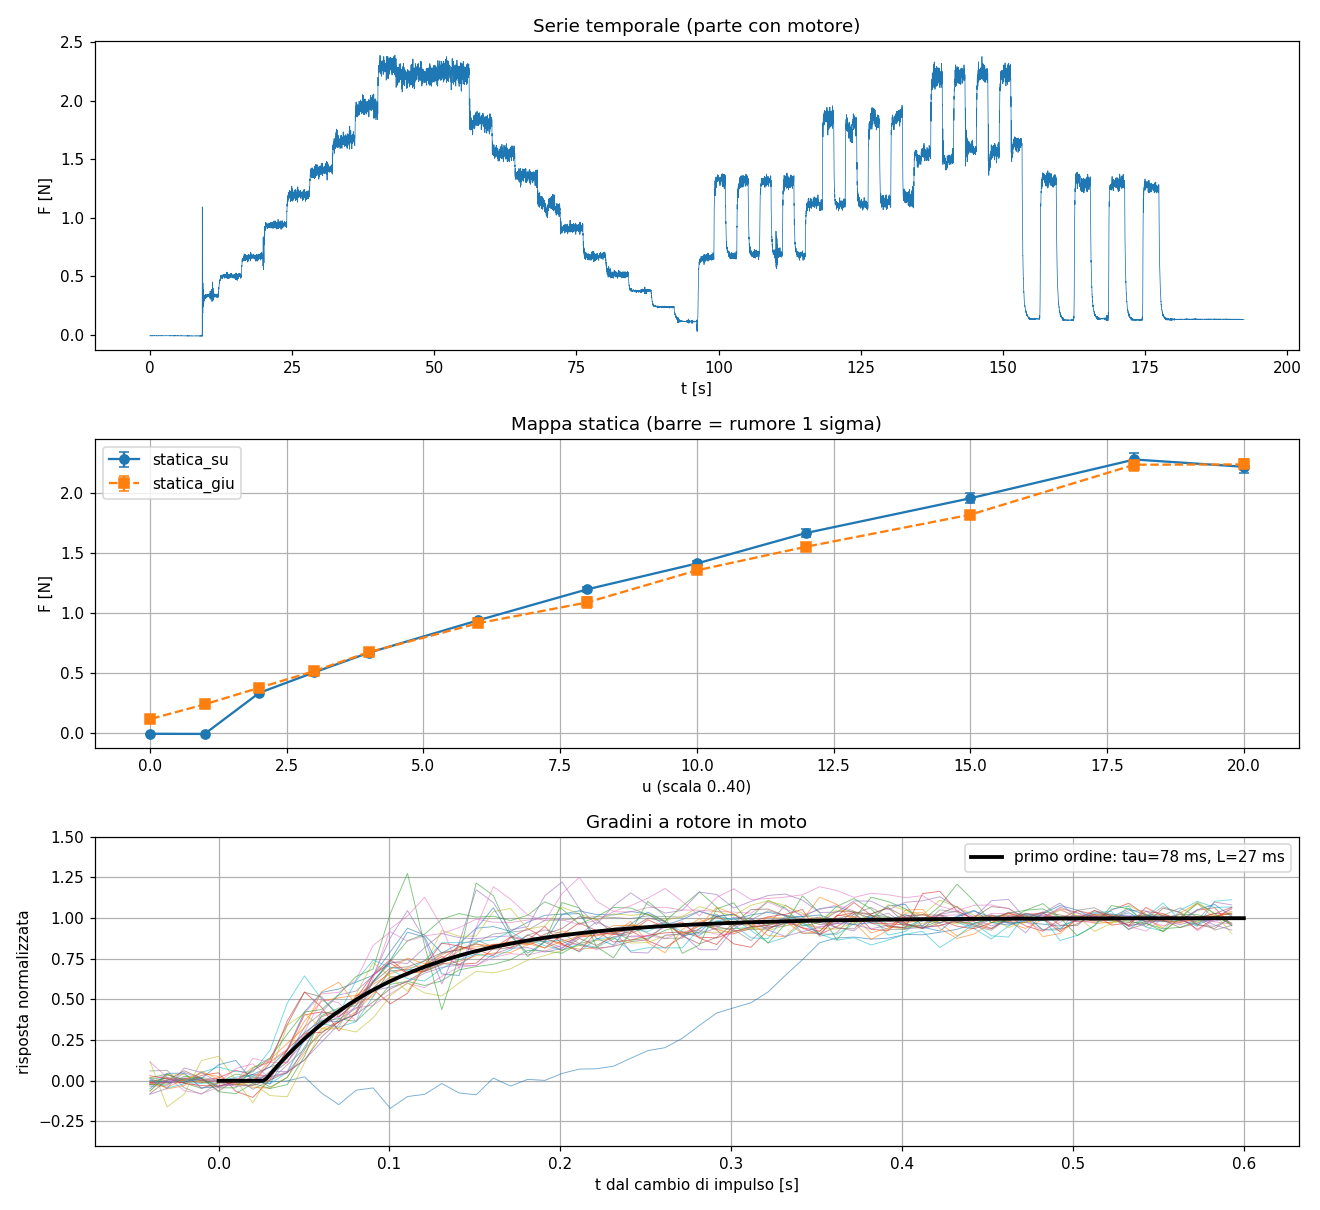
\includegraphics[width=0.92\textwidth]{../img/analisi_sysid.png}
\caption{Test di identificazione: serie temporale, mappa statica (salita e discesa) e gradini a rotore
in moto normalizzati, con il modello del primo ordine sovrapposto.}
\end{figure}

\begin{center}
\begin{tabular}{@{}lll@{}}
\toprule
Grandezza & Simbolo & Valore misurato\\
\midrule
Costante di tempo, rotore in moto & $\tau_{on}$ & 78 ms (33--112 ms tra le ripetizioni)\\
Costante di tempo, spegnimento & $\tau_{off}$ & 174 ms\\
Ritardo puro, rotore in moto & $L$ & 27 ms\\
Ritardo di avvio da fermo & $L_{avvio}$ & 200 ms\\
Soglia di avvio / arresto & $u_{avvio}$, $u_{arresto}$ & 1.5 / 0.5 (scala 0--40)\\
Rumore & $\sigma$ & $1.1\ \text{mN} + 2.08\%\cdot T$\\
Spostamento dello zero dopo i test & $b$ & $+0.132$ N\\
Spinta massima & & $\approx 2.21$ N (saturazione)\\
\bottomrule
\end{tabular}
\end{center}

Mappa statica ``in moto'' (zero sottratto; media di salita e discesa dove il motore gira in entrambe):
\begin{center}
\small
\begin{tabular}{@{}l*{11}{c}@{}}
\toprule
$u$ & 1 & 2 & 3 & 4 & 6 & 8 & 10 & 12 & 15 & 18 & 20\\
$F$ [N] & 0.123 & 0.302 & 0.456 & 0.617 & 0.873 & 1.090 & 1.331 & 1.557 & 1.835 & 2.206 & 2.206\\
\bottomrule
\end{tabular}
\end{center}
La mappa è quasi lineare, circa $0.11$~N per unità di $u$, leggermente concava, e satura a 18.

% =============================================================================
\section{Modello del rotore}

\subsection{Perché un primo ordine}
Il rotore è un'inerzia $J$ accelerata dalla coppia del motore $Q_m$ e frenata dalla coppia
aerodinamica $Q_a(\omega)$:
\begin{equation}
J\dot\omega = Q_m(u,\omega) - Q_a(\omega).
\end{equation}
L'ESC regola la velocità in modo che, a regime, $\omega$ dipenda solo dal comando $u$.
Linearizzando attorno a un punto di lavoro, la deviazione $\delta\omega$ obbedisce a
$J\,\delta\dot\omega = -k_\omega\,\delta\omega + k_u\,\delta u$, cioè a un sistema del primo ordine con
costante di tempo $\tau = J/k_\omega$. Poiché la spinta è una funzione regolare di $\omega$
($T\propto\omega^2$), anche le piccole variazioni di spinta seguono, in prima approssimazione, un primo ordine.

Questa è la giustificazione del modello; la sua validità è stata verificata sui dati: le risposte ai
gradini si sovrappongono bene alla curva di un primo ordine con ritardo (figura precedente).
La dispersione di $\tau$ (33--112 ms) indica che la linearizzazione vale solo localmente: per questo
$\tau$ viene randomizzata in training.

\subsection{Discretizzazione esatta}
Con spinta di regime $T^*(u)$ (dalla mappa statica), il modello continuo è
\begin{equation}
\dot T = \frac{T^* - T}{\tau}.
\end{equation}
Il controllore agisce a passi di $\Delta t = 20$~ms e mantiene il comando costante tra un passo e
l'altro (\emph{zero-order hold}). Su un intervallo con $T^*$ costante la soluzione esatta è
\begin{equation}
T(t_k + \Delta t) = T^* + \big(T(t_k) - T^*\big)e^{-\Delta t/\tau}
\;\Rightarrow\;
\boxed{T_{k+1} = T_k + \alpha\,(T^* - T_k),\qquad \alpha = 1 - e^{-\Delta t/\tau}}
\end{equation}
Con $\tau = 78$~ms: $\alpha = 1 - e^{-0.02/0.078} = 0.226$.

\begin{nota}[Perché non Eulero]
Il metodo di Eulero darebbe $\alpha_E = \Delta t/\tau = 0.256$, un errore del 13\%. Per la $\tau$ più
piccola randomizzata ($\approx40$~ms) l'errore sale al 27\%, e per $\tau < \Delta t/2 = 10$~ms Eulero
diventerebbe addirittura instabile ($\alpha_E>2$). La formula esatta è corretta per ogni $\tau>0$.
\end{nota}

\subsection{Deadband con isteresi e ritardo di avvio}
Dai dati: da fermo il motore parte solo se $u \ge u_{avvio}$, e impiega circa 200~ms a sincronizzarsi
prima di spingere; una volta in moto si ferma solo se $u < u_{arresto} < u_{avvio}$. Si modella come
una macchina a due stati:
\begin{center}
\begin{tabular}{@{}lll@{}}
\toprule
Stato & Condizione & Evoluzione\\
\midrule
fermo & $u \ge u_{avvio}$ per $\mathrm{round}(L_{avvio}/\Delta t) = 10$ passi consecutivi & $\to$ in moto\\
fermo & altrimenti & $T$ decade con $\tau_{off}$ verso 0\\
in moto & $u < u_{arresto}$ & $\to$ fermo\\
in moto & altrimenti & $T$ tende a $g\cdot T^*(u)$ con $\tau_{on}$\\
\bottomrule
\end{tabular}
\end{center}
Il guadagno $g$ (nominale 1) moltiplica la mappa statica; $\tau_{off} > \tau_{on}$ perché in
spegnimento il rotore rallenta solo per attrito e resistenza dell'aria, senza frenata attiva.
\envlines{186}{205}
La funzione \code{np.interp} interpola linearmente la tabella e, oltre l'ultimo punto, restituisce
il valore di bordo: la saturazione a 2.21~N è quindi inclusa automaticamente.

\subsection{Ritardo di attuazione}
Il comando calcolato al passo $k$ raggiunge il motore dopo $n$ passi: si usa una coda FIFO
inizializzata con $n$ zeri. A ogni passo si accoda il nuovo comando e si estrae il più vecchio:
\begin{equation}
u^{applicato}_k = u_{k-n}.
\end{equation}
\envlines{276}{278}
Il ritardo misurato (27~ms) corrisponde a 1--2 passi; sul banco con PC + Arduino il comportamento
in anello chiuso è risultato equivalente a 3 passi (sezione~\ref{sec:esperimenti}). In training $n$
è estratto in $\{1,2,3,4\}$; il valore nominale è 3.

% =============================================================================
\section{Modello della misura e del disturbo}

\subsection{Misura}
Implementa l'equazione~\eqref{eq:misura}. Il rumore è gaussiano con deviazione standard che
cresce con la spinta, perché a motore acceso domina la vibrazione meccanica:
\begin{equation}
n \sim \mathcal{N}(0,\sigma^2),\qquad \sigma = s_0 + s_1\,|T|,\quad s_0 = 1.1\ \text{mN},\ s_1 = 0.0208 .
\end{equation}
A $T = 1.15$~N: $\sigma \approx 25$~mN.
\envlines{207}{212}

\subsection{Disturbo: inclinazione della corsia}
L'inclinazione non è osservata dalla rete. Ogni 100--300 passi (2--6~s) viene estratto un nuovo
angolo in $[-14^\circ, 14^\circ]$, raggiunto con un gradino (probabilità 0.5) o con una rampa
di durata 0.5--3~s.
\envlines{163}{180}

\subsection{Validazione del simulatore}
La stessa sequenza di comandi del test di identificazione è stata data al simulatore (parametri
nominali) e confrontata con la misura: RMS della differenza $0.083$~N, che scende a $0.069$~N
togliendo lo spostamento medio dello zero ($0.047$~N), effetto coperto in training dalla
randomizzazione di $b$.
\begin{figure}[H]
\centering
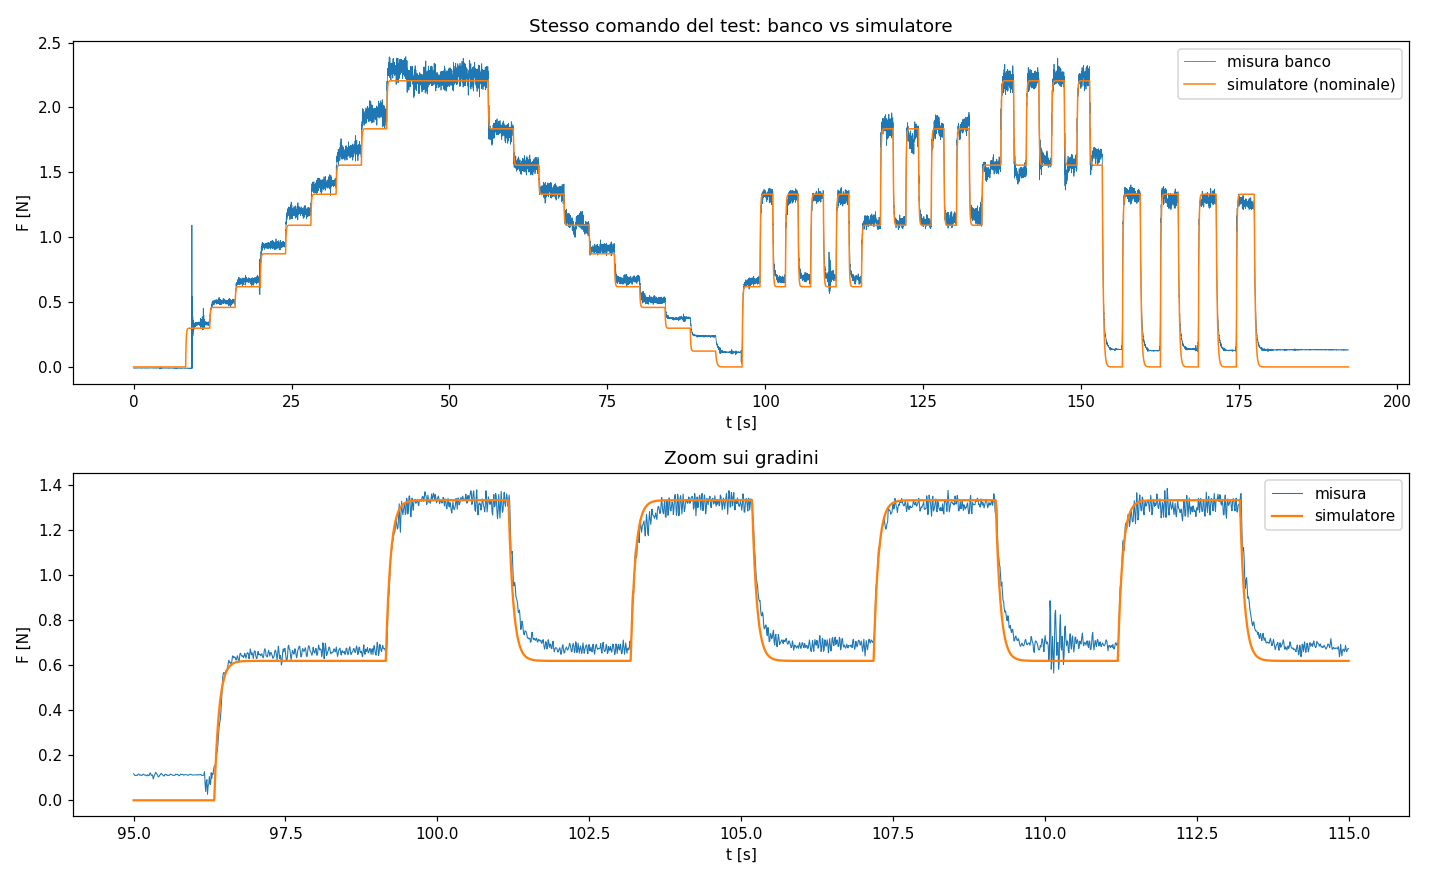
\includegraphics[width=0.92\textwidth]{../img/validazione_simulatore.png}
\caption{Stesso comando dato al banco e al simulatore. In basso, ingrandimento sui gradini.}
\end{figure}

% =============================================================================
\section{Domain randomization}

Il simulatore non sarà mai identico al banco. Invece di un solo modello si addestra la policy su
una famiglia di modelli: a ogni episodio i parametri vengono estratti in intervalli attorno ai
valori misurati. Una policy che funziona su tutta la famiglia ha buone probabilità di funzionare
anche sul banco, purché il banco ``stia dentro'' la famiglia.

\begin{center}
\begin{tabularx}{\textwidth}{@{}llX@{}}
\toprule
Parametro & Intervallo & Motivazione\\
\midrule
massa $m$ & $\times[0.95,\,1.05]$ & pesata: incertezza piccola\\
guadagno $g$ & $[0.85,\,1.15]$ & isteresi salita/discesa, riscaldamento, incertezza di calibrazione della cella\\
$\tau_{on}$ & $\approx[40,\,112]$ ms & dispersione misurata tra le ripetizioni\\
$\tau_{off}$ & $\times[0.85,\,1.15]$ & \\
$u_{avvio}$ & $\times[0.8,\,1.3]$ & \\
$u_{arresto}$ & $\times[0.6,\,1.6]$, $\le u_{avvio}$ & l'isteresi non può invertirsi\\
$L_{avvio}$ & $\times[0.75,\,1.25]$ & \\
ritardo $n$ & $\{1,2,3,4\}$ passi & 20--80 ms: contiene i $\approx$60 ms visti sul banco con margine\\
rumore $s_1$ & $\times[0.7,\,1.5]$ & \\
bias $b$ & $[-0.05,\,0.18]$ N & lo zero misurato si sposta fino a $+0.13$ N\\
\bottomrule
\end{tabularx}
\end{center}
\envlines{127}{157}

\begin{attenzione}[Lezione dalla policy E]
La randomizzazione deve contenere la realtà \emph{con margine}. La policy E era stata addestrata con
ritardo di 1--2 passi; sul banco il ritardo era circa 3 passi e la policy oscillava a $\approx3$~Hz.
\end{attenzione}

% =============================================================================
\section{Formulazione come problema di RL}

\subsection{Il ciclo}
A ogni passo $k$ ($\Delta t = 20$~ms): l'ambiente fornisce l'osservazione $o_k$, la policy sceglie
l'azione $a_k$, il simulatore avanza e restituisce la ricompensa $r_k$. Un episodio dura
1000 passi (20~s) e parte con motore fermo e inclinazione casuale.
\envlines{268}{313}

\subsection{Azione}
La rete produce $a\in[-1,1]$. La conversione nel comando del banco è
\begin{equation}
c = c_{min} + (1 - c_{min})\,\frac{a+1}{2}\in[c_{min},1],\qquad u = c\,u_{max},
\qquad c_{min} = 0.05,\ u_{max} = 20 .
\end{equation}
Quindi $u\in[1,\,20]$: il minimo è sopra la soglia di arresto ($0.5$), così la rete non può spegnere
il motore (una ripartenza costerebbe 200~ms), e il massimo è il punto in cui la mappa satura.

\subsection{Osservazione}
\begin{center}
\begin{tabularx}{\textwidth}{@{}clX@{}}
\toprule
\# & Grandezza & Perché\\
\midrule
0 & $F_{lc}/2.5$ & forza misurata; 2.5 N $\approx$ spinta massima, così il valore sta circa in $[0,1]$\\
1 & $e/F_{ref}$, con $e = F_{ref} - F_{lc}$ & errore normalizzato: la quantità da annullare\\
2 & $\widehat{\Delta F}/2.5$ & variazione della forza filtrata: informa sulla tendenza\\
3--5 & $c_{k-1},\,c_{k-2},\,c_{k-3}$ & ultimi tre comandi: con il ritardo di attuazione fanno parte dello stato\\
6 & $I/I_{max}$ & integrale dell'errore: permette di eliminare l'errore a regime\\
\bottomrule
\end{tabularx}
\end{center}
\envlines{219}{232}

\paragraph{Filtro della derivata.} La differenza tra due misure consecutive è dominata dal rumore.
Si usa un filtro esponenziale (EMA):
\begin{equation}
\widehat{\Delta F}_k = \widehat{\Delta F}_{k-1} + \beta\big((F_k - F_{k-1}) - \widehat{\Delta F}_{k-1}\big),\qquad \beta = 0.2,
\end{equation}
equivalente a un passa-basso del primo ordine con costante di tempo
$\tau_{EMA} = -\Delta t/\ln(1-\beta) = 0.02/0.223 \approx 90$~ms.
Per un ingresso a rumore bianco la varianza in uscita è ridotta del fattore $\beta/(2-\beta) = 0.11$.

\paragraph{Integrale con anti-windup.}
\begin{equation}
I_k = \mathrm{clip}\big(I_{k-1} + e_k\,\Delta t,\ -I_{max},\ I_{max}\big),\qquad I_{max} = 0.5\ \text{N\,s}.
\end{equation}
La saturazione impedisce che, durante una saturazione del motore, l'integrale cresca senza limite.
Il valore di $I_{max}$ fissa anche la \emph{sensibilità} dell'osservazione: con un errore di 0.1~N,
$I/I_{max}$ cresce di $0.1/0.5 = 0.2$ al secondo. Con il valore iniziale $I_{max} = 2$ cresceva di
appena $0.05$ al secondo, un segnale troppo debole perché la rete lo usasse (esperimento E).

\paragraph{Storia dei comandi e proprietà di Markov.}
Il RL presuppone che l'osservazione contenga tutto ciò che serve a prevedere il futuro (proprietà di
Markov). Con un ritardo di $n$ passi, i comandi $c_{k-1},\dots,c_{k-n}$ sono già stati inviati ma non
hanno ancora avuto effetto sulla forza: senza vederli la rete non sa che una correzione è ``in
viaggio'' e ne aggiunge un'altra, innescando un'oscillazione. Tre comandi coprono il ritardo nominale.

\subsection{Ricompensa}
\begin{equation}
r = -e_n^2 - w_{e1}\,|e_n| - w_{\Delta}\,(\Delta c)^2 - w_u\,c^2,
\qquad e_n = \frac{e}{F_{ref}},\quad w_{e1} = 1,\ w_\Delta = 5,\ w_u = 0.01 .
\end{equation}
\begin{itemize}
\item $e_n^2$: penalizza molto gli errori grandi. Vicino a zero però è quasi piatto (derivata $2e_n\to0$).
\item $|e_n|$: derivata costante. Con un errore persistente di 0.15~N, $e_n = 0.130$:
  il termine quadratico costa $0.017$ a passo, quello lineare $0.130$, circa 8 volte di più.
  Senza il termine lineare la policy lasciava errori di questo tipo (esperimento A).
\item $(\Delta c)^2$: penalizza un comando che cambia molto da un passo all'altro (usura, rumore, vibrazioni).
\item $c^2$: piccola penalità sullo sforzo, rompe la simmetria a favore di comandi bassi a parità di errore.
\end{itemize}
Normalizzare l'errore su $F_{ref}$ rende i pesi indipendenti dalle unità di misura.

% =============================================================================
\section{L'algoritmo SAC}

\subsection{Obiettivo}
Nel RL classico si cerca la policy $\pi$ che massimizza il ritorno scontato atteso
$\mathbb{E}\big[\sum_k \gamma^k r_k\big]$. Il fattore $\gamma$ fissa l'orizzonte efficace,
\begin{equation}
H \approx \frac{1}{1-\gamma} = 100\ \text{passi} = 2\ \text{s}\qquad(\gamma = 0.99),
\end{equation}
scelto perché l'errore lasciato da un cambio di inclinazione dura secondi: con $\gamma = 0.98$
($H = 1$~s) il beneficio di correggerlo era poco visibile alla policy.

SAC (\emph{Soft Actor-Critic}) massimizza un obiettivo che premia anche l'entropia della policy:
\begin{equation}
J(\pi) = \mathbb{E}\Big[\sum_k \gamma^k\big(r_k + \alpha\,\mathcal{H}(\pi(\cdot\,|\,s_k))\big)\Big],
\qquad \mathcal{H}(\pi(\cdot|s)) = -\mathbb{E}_{a\sim\pi}[\log\pi(a|s)] .
\end{equation}
Il termine di entropia, pesato dalla temperatura $\alpha$, spinge a esplorare e impedisce che la
policy diventi deterministica troppo presto.

\subsection{Critic: la Q ``soft''}
Il critic stima $Q(s,a)$, il ritorno atteso partendo da $s$ con l'azione $a$ e poi seguendo $\pi$.
Per l'obiettivo con entropia vale l'equazione di Bellman ``soft'':
\begin{equation}
Q(s,a) = r + \gamma\,\mathbb{E}_{s',\,a'\sim\pi}\big[Q(s',a') - \alpha\log\pi(a'|s')\big].
\end{equation}
Si usano due reti critic $Q_{\phi_1}, Q_{\phi_2}$ e, per il bersaglio, il minimo delle due versioni
``lente'' (\emph{target network}) $Q_{\bar\phi_j}$, per ridurre la sovrastima sistematica di $Q$:
\begin{equation}
y = r + \gamma\Big(\min_{j=1,2} Q_{\bar\phi_j}(s',a') - \alpha\log\pi(a'|s')\Big),\quad a'\sim\pi(\cdot|s'),
\qquad \mathcal{L}_Q = \mathbb{E}\big[(Q_{\phi_j}(s,a) - y)^2\big].
\end{equation}
Le reti target seguono quelle principali con una media mobile:
$\bar\phi \leftarrow \tau_p\,\phi + (1-\tau_p)\,\bar\phi$, $\tau_p = 0.005$.

\subsection{Actor e trucco della riparametrizzazione}
L'actor produce media $\mu_\theta(s)$ e deviazione standard $\sigma_\theta(s)$ di una gaussiana, poi
schiaccia con $\tanh$ per stare in $[-1,1]$. Per poter derivare rispetto a $\theta$ attraverso il
campionamento si scrive l'azione come funzione deterministica di un rumore esterno:
\begin{equation}
a = \tanh\big(\mu_\theta(s) + \sigma_\theta(s)\,\varepsilon\big),\qquad \varepsilon\sim\mathcal{N}(0,1).
\end{equation}
L'actor minimizza
\begin{equation}
\mathcal{L}_\pi = \mathbb{E}_{s,\varepsilon}\Big[\alpha\log\pi_\theta(a|s) - \min_{j} Q_{\phi_j}(s,a)\Big],
\end{equation}
cioè cerca azioni con $Q$ alto mantenendo la distribuzione larga.

\paragraph{Correzione della $\tanh$.} Se $z\sim\mathcal{N}(\mu,\sigma^2)$ e $a = \tanh z$, per il
cambio di variabile di una densità
\begin{equation}
\pi(a|s) = \mathcal{N}(z;\mu,\sigma^2)\left|\frac{da}{dz}\right|^{-1}
\;\Rightarrow\;
\log\pi(a|s) = \log\mathcal{N}(z;\mu,\sigma^2) - \log\big(1 - \tanh^2 z\big).
\end{equation}
Senza questo termine l'entropia sarebbe calcolata sulla gaussiana e non sull'azione vera, e la
policy verrebbe premiata per spingere $z$ verso valori enormi (azioni saturate a $\pm1$).

\subsection{Temperatura automatica}
Invece di fissare $\alpha$ a mano, SAC la regola per mantenere l'entropia attorno a un valore
obiettivo $\bar{\mathcal{H}}$ (in Stable-Baselines3: $-\dim(\mathcal{A}) = -1$):
\begin{equation}
\mathcal{L}_\alpha = \mathbb{E}_{a\sim\pi}\big[-\alpha\,(\log\pi(a|s) + \bar{\mathcal{H}})\big].
\end{equation}
Se l'entropia è sotto l'obiettivo, $-\log\pi < \bar{\mathcal{H}}$, il gradiente fa crescere $\alpha$
(più premio all'esplorazione), e viceversa: è un anello di controllo sull'entropia.

\subsection{Off-policy e replay buffer}
SAC è \emph{off-policy}: ogni transizione $(s,a,r,s')$ viene salvata in un buffer (200\,000 elementi)
e le reti vengono aggiornate su minibatch estratti a caso dal buffer, anche se raccolti con versioni
precedenti della policy. Questo rende SAC molto più efficiente nei campioni dei metodi on-policy.

\subsection{Configurazione usata}
\envlines{357}{369}
\begin{center}
\begin{tabular}{@{}lll@{}}
\toprule
Iperparametro & Valore & Origine\\
\midrule
learning rate & $3\cdot10^{-4}$ & impostato\\
buffer & 200\,000 & impostato\\
batch & 256 & impostato\\
$\gamma$ & 0.99 & impostato\\
passi di training & 300\,000 & impostato\\
reti actor e critic & $2\times256$, ReLU & default SB3\\
numero di critic & 2 & default SB3\\
$\tau_p$ (target) & 0.005 & default SB3\\
$\alpha$ & automatica, $\bar{\mathcal{H}} = -1$ & default SB3\\
\bottomrule
\end{tabular}
\end{center}
Durante il training un \code{EvalCallback} valuta la policy ogni 5000 passi su 5 episodi
\emph{nominali} con azioni deterministiche, e salva il modello migliore in
\code{best\_sac\_fan/best\_model.zip}.

% =============================================================================
\section{Esperimenti}
\label{sec:esperimenti}

\subsection{Metriche}
Il reward cambia da un esperimento all'altro, quindi non è confrontabile: si confrontano metriche
fisiche, su 20 episodi randomizzati con semi fissi (gli stessi per tutte le policy), escludendo i
primi 2~s (avvio):
\begin{itemize}
\item \textbf{RMS} dell'errore di forza;
\item \textbf{offset lento}: valore medio assoluto dell'errore filtrato con un filtro mediano di 1~s
  (l'errore che resta dopo un cambio di inclinazione);
\item \textbf{oscillazione}: deviazione standard dell'errore meno la sua componente lenta;
\item $\overline{|\Delta c|}$: variazione media del comando per passo;
\item spegnimenti del motore per episodio.
\end{itemize}

\subsection{Risultati}
\begin{center}
\small
\begin{tabularx}{\textwidth}{@{}lXccccc@{}}
\toprule
Esp. & Modifica & RMS [N] & Offset [N] & Oscill. [N] & $\overline{|\Delta c|}$ & Spegn.\\
\midrule
A & modello dalla sysid, reward $e_n^2$, $\gamma$ 0.98, 150k passi & 0.136 & 0.106 & 0.057 & 0.012 & 0\\
D & + termine $|e_n|$, $\gamma$ 0.99, 300k passi & 0.117 & 0.085 & 0.061 & 0.021 & 0.25\\
E & + $I_{max}$ $2\to0.5$, $c_{min} = 0.05$ & 0.090 & 0.049 & 0.059 & 0.016 & 0\\
\bottomrule
\end{tabularx}
\end{center}
In condizioni nominali: A 0.127~N, D 0.108~N, E 0.078~N.

\begin{figure}[H]
\centering
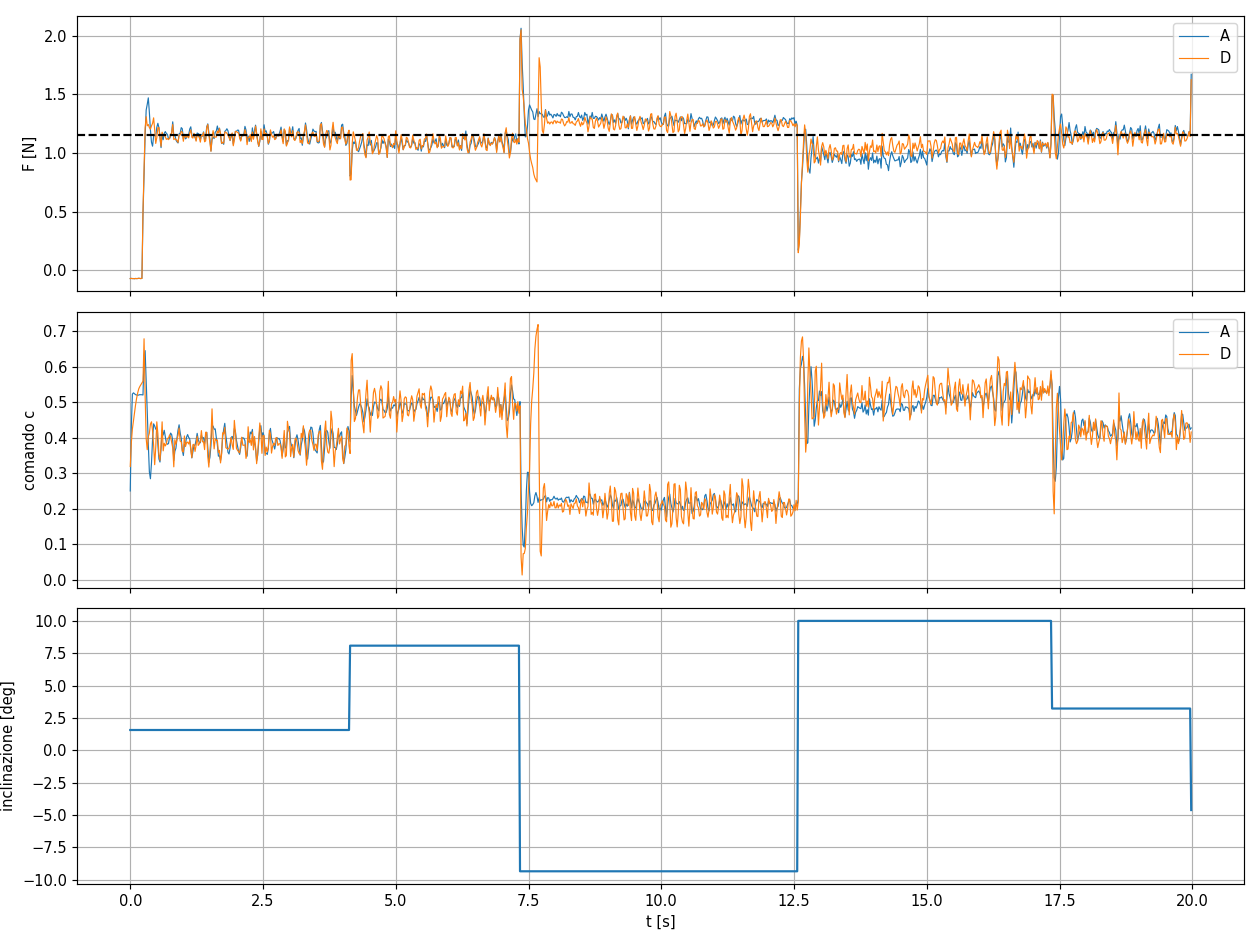
\includegraphics[width=0.48\textwidth]{../img/confronto_A_D.png}\hfill
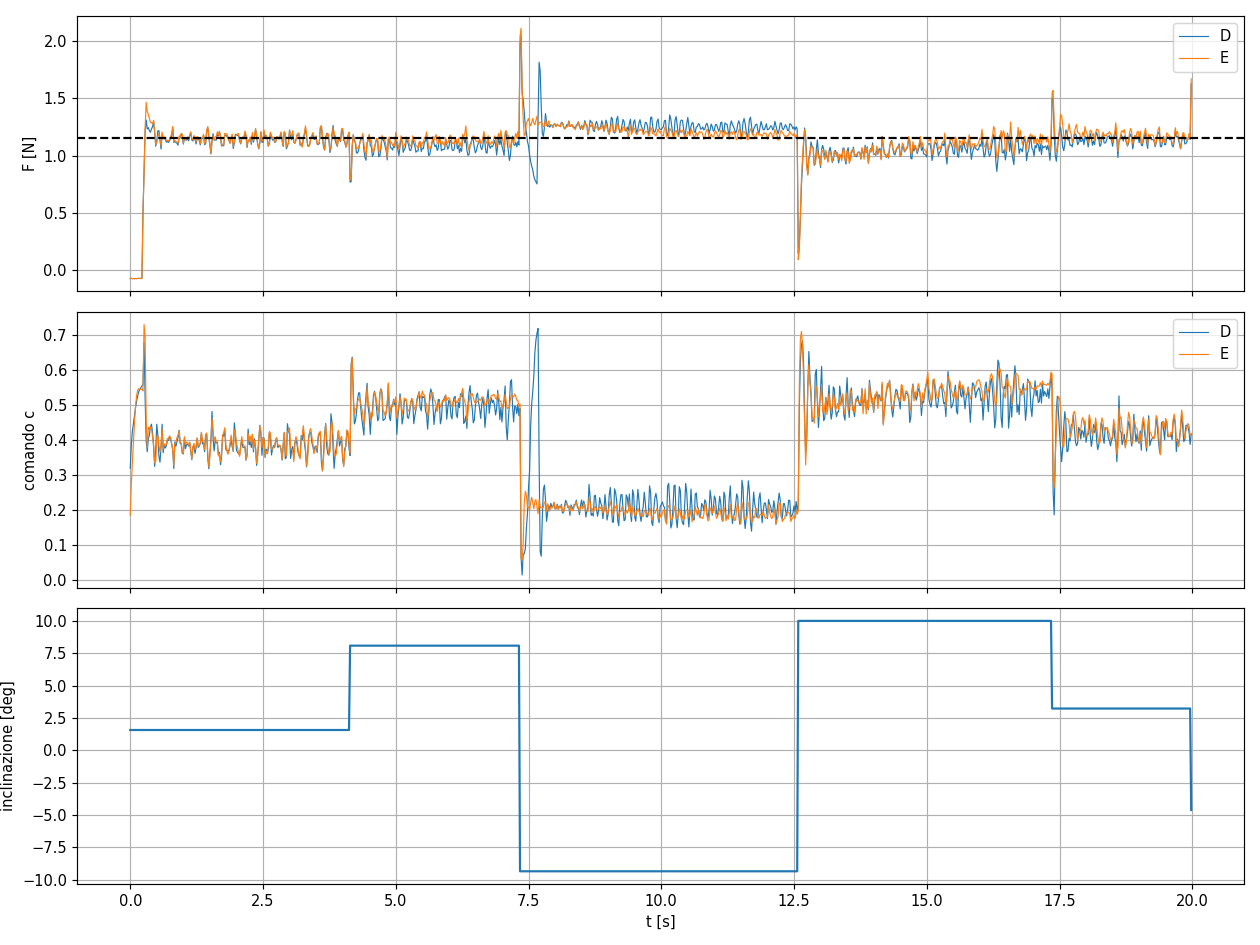
\includegraphics[width=0.48\textwidth]{../img/confronto_D_E.png}
\caption{Stesso episodio randomizzato: A contro D (sinistra) e D contro E (destra).}
\end{figure}

\paragraph{A $\to$ D (reward shaping).} Il termine lineare riduce l'offset del 20\%, ma rende
relativamente più conveniente muovere il comando: $\overline{|\Delta c|}$ cresce del 75\% e compaiono
spegnimenti del motore (la policy portava il comando quasi a zero per correggere un overshoot).

\paragraph{D $\to$ E (scala delle osservazioni e vincolo sull'azione).} Rendere l'integrale 4 volte
più sensibile dimezza l'offset senza cambiare rete né reward; $c_{min}$ elimina gli spegnimenti.
È stato il miglioramento più grande.

\subsection{Sul banco: la policy E}
\begin{figure}[H]
\centering
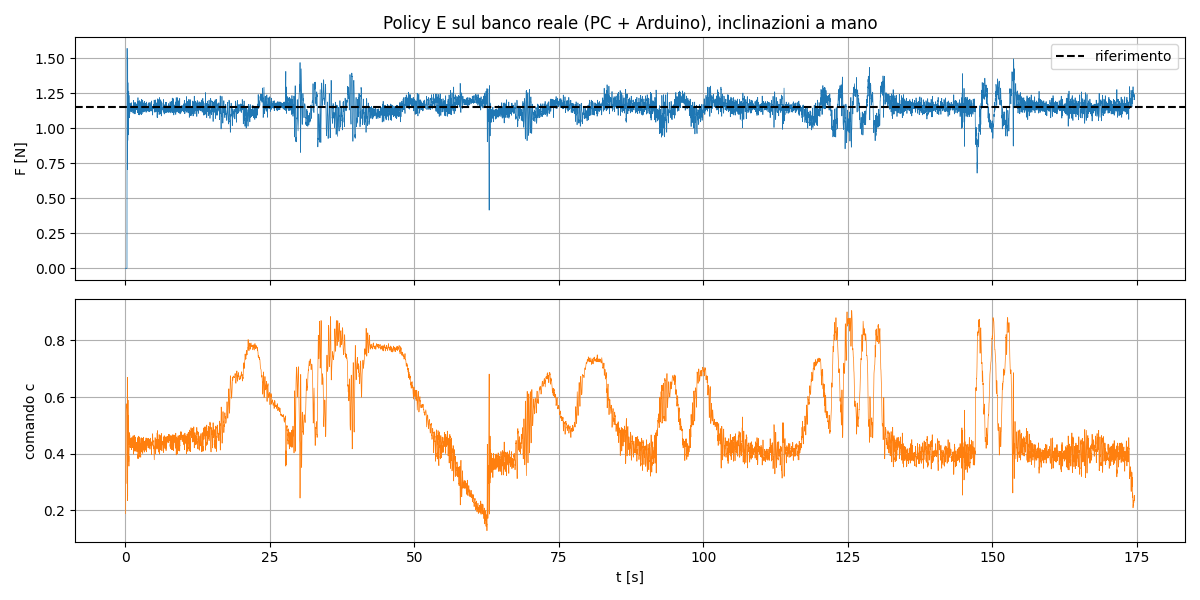
\includegraphics[width=0.85\textwidth]{../img/prova_reale_E.png}
\caption{Policy E sul banco reale (PC + Arduino), 175 s con inclinazioni a mano.}
\end{figure}
RMS 0.067~N sulla prova da 175~s (0.022--0.030~N nei tratti a corsia ferma), errore medio
$+0.003$~N: prestazioni nell'intervallo previsto dalla simulazione. Però la FFT dell'errore mostrava
un picco a $\approx3$~Hz (fino al 47\% della varianza tra 2 e 5~Hz in una prova breve), presente
anche nel comando: un'oscillazione d'anello. In simulazione la policy E riproduce lo stesso spettro
con un ritardo di 3 passi, e diventa quasi instabile con 4.

\subsection{Esperimento F: robustezza al ritardo}
Modifiche: ritardo randomizzato in $\{1,\dots,4\}$ passi e ultimi tre comandi nell'osservazione.
Valutazione con il ritardo forzato a ogni valore (12 episodi randomizzati per caso):
\begin{center}
\small
\begin{tabular}{@{}lcccccc@{}}
\toprule
Ritardo & \multicolumn{2}{c}{RMS [N]} & \multicolumn{2}{c}{Quota 2--5 Hz} & \multicolumn{2}{c}{$\overline{|\Delta c|}$}\\
 & E & F & E & F & E & F\\
\midrule
1 passo (20 ms)  & \textbf{0.089} & 0.096 & 11\% & 8\%  & 0.016 & 0.013\\
2 passi (40 ms)  & \textbf{0.101} & 0.105 & 20\% & 12\% & 0.020 & 0.014\\
3 passi (60 ms)  & 0.151 & \textbf{0.111} & 56\% & \textbf{20\%} & 0.032 & \textbf{0.014}\\
4 passi (80 ms)  & 0.237 & \textbf{0.118} & 76\% & \textbf{26\%} & 0.045 & \textbf{0.014}\\
\bottomrule
\end{tabular}
\end{center}
\begin{figure}[H]
\centering
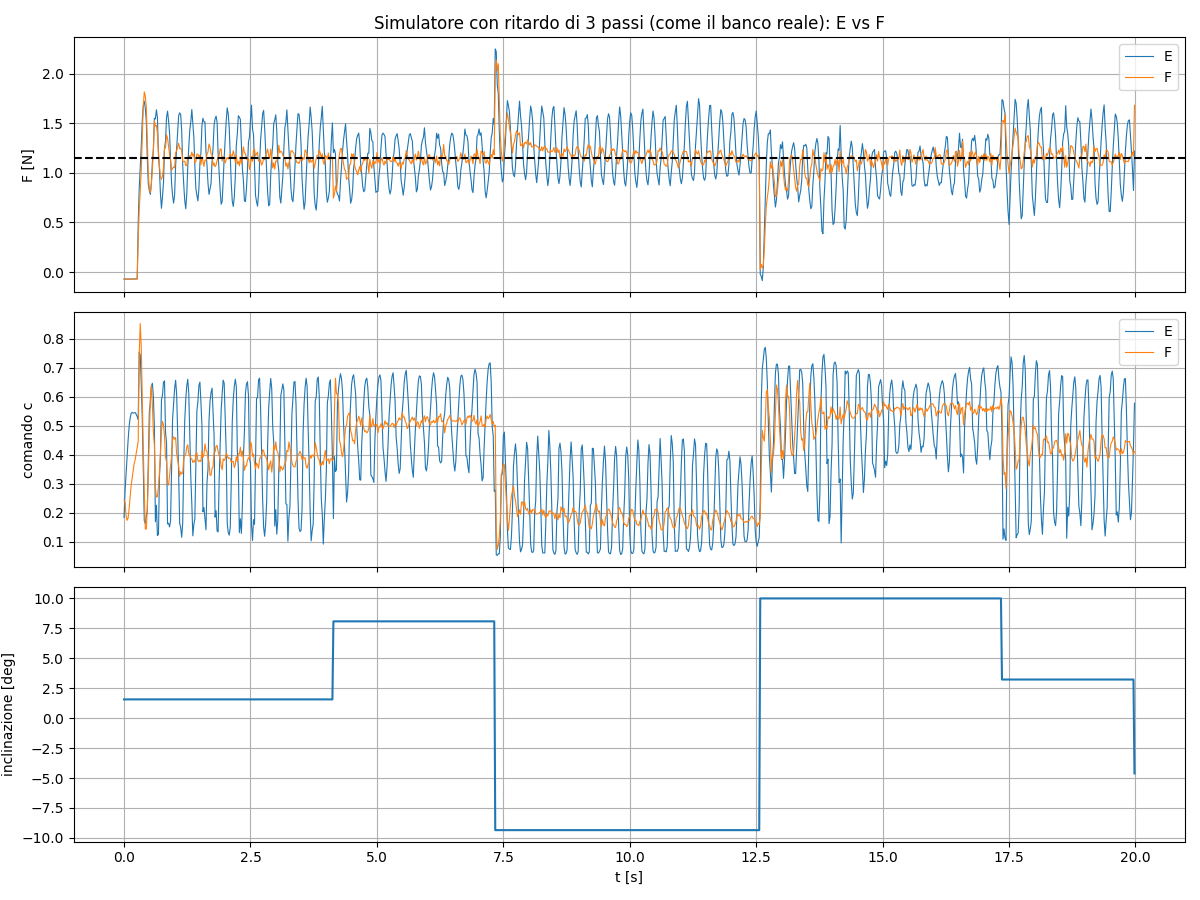
\includegraphics[width=0.8\textwidth]{../img/confronto_E_F_ritardo3.png}
\caption{E contro F nello stesso episodio con ritardo di 3 passi.}
\end{figure}
Con il ritardo del banco F ha il 26\% di errore in meno e circa un terzo dell'oscillazione; al
crescere del ritardo peggiora poco, mentre E si avvicina all'instabilità. Il prezzo è una leggera
perdita con ritardo piccolo: il compromesso tra robustezza e prestazioni nominali.
Il miglior modello F è stato salvato a 110\,000 passi.

\begin{nota}[Policy F sul banco]
La policy F è stata provata sul banco con PC + Arduino con esito positivo (osservazione diretta
durante la prova). Il file della prova non è stato archiviato nel repository: il confronto
quantitativo con E sul banco resta da fare con il protocollo di \code{docs/05\_prove\_sul\_banco.md}.
\end{nota}

% =============================================================================
\section{Riepilogo delle lezioni}
\begin{itemize}
\item Il simulatore va costruito sui dati del banco e validato confrontandolo con il banco a parità
  di comando, prima di addestrare.
\item Il dimensionamento del compito (riferimento, angolo massimo) va fatto sui limiti fisici
  misurati, altrimenti la policy impara solo a saturare.
\item Discretizzare la dinamica in modo esatto: è semplice e vale per ogni costante di tempo.
\item La randomizzazione deve contenere la realtà con margine, in particolare sul ritardo.
\item Con un ritardo, l'osservazione deve contenere i comandi non ancora arrivati (proprietà di Markov).
\item La scala delle osservazioni conta quanto il reward: un segnale che varia poco è quasi invisibile alla rete.
\item Vincolare lo spazio delle azioni (qui $c_{min}$) può eliminare comportamenti dannosi senza toccare il reward.
\item Confrontare policy con metriche fisiche e semi fissi, mai con il reward se il reward è cambiato.
\end{itemize}

% =============================================================================
\appendix
\section{Codice: parametri e costruttore dell'ambiente}
\envlines{41}{58}
\envlines{65}{121}

\section{Codice: reset dell'episodio}
\envlines{238}{262}

\end{document}
